\section{Symbolic model checking}
\SetKwProg{Fn}{function}{:}{}
\SetKwInput{KwIn}{In}
\SetKwInput{KwOut}{Out}
\newcommand{\safety}{\textsc{Safety}\xspace}
In this section, we present the \safety problem and the state-of-the-art algorithm IC3/ \spc. They are needed for understanding \cref{chap:dopey}.
\paragraph{The \safety problem.}
% \nl{currently borrowed from gspacer}

% \textbf{Safety problem of transition system}
We consider first order logic modulo theories, using the standard notation and terminology. A first-order language modulo theory $\cT$ is defined over a signature $\Sig$ containing constant, function, and predicate symbols. 

A \emph{transition system} is a tuple $\langle \Sig, \Init,
\Tr \rangle$.
$\Sig$, $\Sig'$, and $\Sig^i$ are used to present the pre-state, the post-state, and the state of the system after executing $i$ steps, respectively ($\Sig' = \{v' \mid v \in \Sig\}$, $\Sig^i = \{v^i \mid v \in \Sig\}$). 
$\Init$ is a formula over $\Sig$ and $\Tr$ is a formula over $\Sig \cup \Sig'$. For a formula $\varphi$ over variables in $\Sig$, we denote by $\varphi'$ the formula obtained by substituting each $v \in \varphi$ by $v' \in \Sig'$, and $\varphi^i$ the formula obtained by substituting each $v \in \varphi$ by $v^i \in \Sig^i$. We also denote $\Tr^i$ a formula obtained by substituting each $v \in \Tr$ by $v^i \in \Sig^i$ and each $v' \in \Tr'$ by $v^{i+1} \in \Sig^{i+1}$.


For simplicity, we omit $\Sig$ and use the shorthand $\trinit$ to represent the
transition system whenever the context is clear.
% \footnote{In fact, a
%   primed copy is introduced in $\Sig'$ only for the uninterpreted symbols in
%   $\Sig$. Interpreted symbols remain the same in $\Sig'$.} 
% The states of the system correspond
% to structures over $\Sig$, 
% $\Init$ represents the initial state and $\Tr$
% represents the transition relation, where $\Sig$ is used to represent the pre-state of a transition, and $\Sig'$ is used to represent the post-state. 

A \emph{\safety problem} is a triple 
$P = \langle \Init, \Tr, \Bad \rangle$, where
$\langle \Init, \Tr \rangle$ is a transition system and $\Bad$ is a
formula over $\Sig$ representing a set of bad states. $P$ is \unsafe if and only
if there exists a number $N$ such that the following is satisfiable:
\begin{align}
\label{form:safety}
    \Init^0\land (\bigwedge^{N-1}_{i=0}Tr^i)\land \Bad^N
\end{align}
In this case, we also say that $P$ has a \emph{counterexample (CEX)} of length $N$. Vice versa, $P$ is \safe if and only if \cref{form:safety} is unsatisfiable.



The \safety problem defined above is an instance of a more general problem,
CHC-SAT, of satisfiability of Constrained Horn Clauses (CHC). With abuse of
notation, in this thesis we use \textit{solving CHCs} and \textit{verifying
  safety properties} interchangeably.

\paragraph{Induction, safe inductive invariant, relative induction, inductive trace.}
A formula $\varphi$ is called an \emph{inductive invariant} of a transition
system $\trinit$ if and only if:
\begin{align}
  \Init &\implies \varphi\\
  \varphi \land \Tr &\implies \varphi'
\end{align}

We also say that a formula $\varphi$ is \emph{inductive relative} to a formula
$F$ if it satisfies initiation and $\varphi \land F \land \Tr \implies \varphi'$.

An inductive invariant $\varphi$ is \safe if:
\begin{align}
  \varphi \implies \lnot \Bad
\end{align}

An \emph{inductive trace} of a transition system is a list of formulas $F = [F_0, F_1, \dots, F_N]$ such
that
\begin{align}
  \Init &\implies F_0 \\
  \forall 0 \leq i < N , F_i \land \Tr &\implies F_{i+1}
\end{align}
We call $F_i$ a \emph{frame}, and we represent each frame $F_i$ as a set of \emph{lemmas}, and each lemma $\ell \in
F_i$ is a clause.

\paragraph{Craig Interpolation.} Given an unsatisfiable formula $A \land B$, a \emph{Craig
interpolant}, denoted $\itp(A,B)$, is a formula $I$ over the shared signature of
$A$ and $B$ such that $A \limp I$ and $I \limp \neg B$.

\begin{figure*}[t]
  \centering
  \begin{subfigure}[b]{0.3\textwidth}
    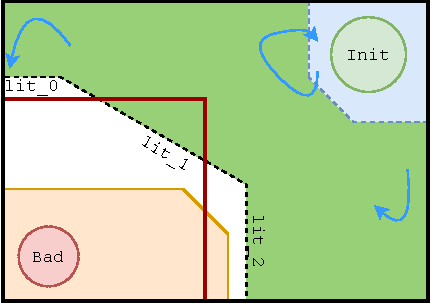
\includegraphics[width=0.99\textwidth]{figures/doping-lemma.pdf}
    \caption{An inductive lemma L = \{\texttt{lit\_0}, \texttt{lit\_1}, \texttt{lit\_2}\}}
    \label{fig:lemma}
	\end{subfigure}
	\begin{subfigure}[b]{0.3\textwidth}
    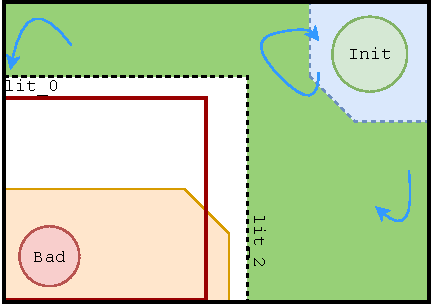
\includegraphics[width=0.99\textwidth]{figures/doping-lemma_gen.pdf}
    \caption{L is successfully generalized by dropping \texttt{lit\_1}}
    \label{fig:ind_gen}
	\end{subfigure}
	\begin{subfigure}[b]{0.3\textwidth}
    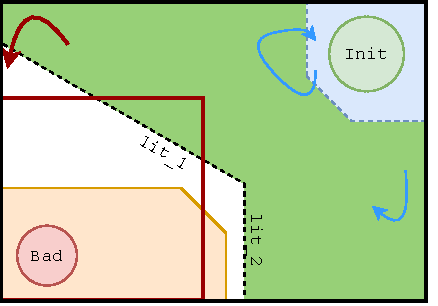
\includegraphics[width=0.99\textwidth]{figures/doping-lemma_not_ind.pdf}
    \caption{L no longer inductive by dropping \texttt{lit\_0}}
    \label{fig:not_ind_gen}
	\end{subfigure}

  \caption{Visualization of inductive generalization.}
  \label{fig:vis_ind_gen}
\end{figure*}




\paragraph{IC3/\spc.}
The current state-of-the-art algorithm to solve CHC is IC3/\spc \cite{spacer}.
At the high level, the main IC3/\spc loop tries to find a CEX of length $N$,
and terminates if the CEX is found (\unsafe), or the lemma that proves such CEX
doesn't exist is also a safe inductive invariant (\safe). 

There are many ways to represent the \spc algorithm, and in this thesis we borrows
the presentation used in \cite{GSpacer}.

\cref{alg:spc} presents the key ingredients of \spc as a set of rules. It
maintains the following:
\begin{itemize}
  \item The current unrolling depth $N$ at
    which a counterexample is searched (there are no counterexamples with depth less
    than $N$).
  \item An inductive trace $F = [F_0, F_1, \ldots]$.
    Intuitively, each frame $F_i$ is a candidate inductive invariant s.t.
    $F_i$ over-approximates states reachable up to $i$ steps from $\Init$.

  \item A queue of \emph{proof obligations} $Q$, where each proof obligation
    (\pob) in $Q$ is a pair $\langle \varphi, i \rangle$ of a cube $\varphi$ and a
    level number $i$, $0 \leq i \leq N$.
    Each \pob $\langle \varphi, i \rangle$ in $Q$ corresponds to a suffix of a potential
    counterexample that has to be blocked in $F_i$, i.e., has to be proven unreachable in $i$ steps.
  \item An under-approximation $\cU$ of reachable
    states, represented as a disjunction.
\end{itemize}

The \texttt{Candidate} rule adds a \pob $\langle \Bad, N \rangle$ to
the queue. If a \pob $\langle \varphi, i \rangle$ cannot be blocked because
$\varphi$ is reachable from frame $(i-1)$, \texttt{Predecessor}
generates a predecessor $\psi$ of $\varphi$ using \getP, and add $\langle \psi,
i-1 \rangle$ to $Q$. \texttt{Successor} updates the set of reachable
states if the \pob is reachable. If the \pob is blocked, \texttt{Conflict}
strengthens the trace $F$ by using interpolation to learn a new lemma
$\ell$ that blocks the \pob, i.e., $\ell \implies \neg \varphi$. \texttt{Induction} 
strengthens a lemma by inductive generalization and \texttt{Propagate} pushes a lemma to a higher frame. If the $\Bad$ state
has been blocked at $N$, \texttt{Unfold} increments the depth of unrolling $N$.
\begin{algorithm2e}[t]
  \SetAlgoNoLine
  \LinesNotNumbered
  \SetKwIF{Guard}{Guard1}{Guard2}{$[$}{$]$}{}{}{}
  \SetKwComment{Rule}{}{}
  \SetKwFor{select}{forever do}{}{}
  \Fn{\spc}{
    \Indm
    \KwIn{$\langle \Init, \Tr, \Bad \rangle$}
    \KwOut{$\langle \safe, \Inv \rangle$ or \unsafe}
    $Q := \emptyset$ \tcp*{\pob queue}
    $N := 0$ \tcp*{maximum safe level}
    $F_0 := \Init, F_i := \top \textbf{ for all } i > 0$ \tcp*{lemma trace}
    $\cU := \Init$ \tcp*{reachable states}
    \select{}{
      \Rule*[h]{Candidate} \lGuard {$\isSat(F_N \land \Bad)$} {
        
        $\qquad Q := Q \cup
        \langle \Bad, N \rangle$}

      \Rule*[h]{Predecessor} \lGuard {$\langle \varphi, i + 1 \rangle \in Q$, $M \models
        F_i \land \Tr \land \varphi'$}{

        $\qquad Q := Q \cup \langle \getP(\varphi, M), i \rangle$}


      \Rule*[h]{Successor} \lGuard {$\langle \varphi, i + 1 \rangle \in Q$, $M \models \cF(\cU) \land
        \varphi'$}{

        $\qquad \cU := \cU \lor  \getS(\cU, M)[\Consts' \mapsto\Consts]$}

      \Rule*[h]{Conflict} \lGuard {$\langle \varphi, i + 1 \rangle \in Q$, $\cF(F_i) \limp \neg \varphi'$}
      {

        $\qquad F_j := ( F_j \land  \itp(\cF(F_i), \varphi')[\Consts' \mapsto \Consts] )
        \makebox[0pt][l]{ $\textbf{ for all } j \leq i + 1 $}$}

      \Rule*[h]{Induction} \lGuard{$\ell \in F_{i+1}, \ell = (\varphi \lor \psi), \cF(\varphi \land F_i) \limp
        \varphi'$}{

        $\qquad F_{j} \gets F_{j} \land \varphi \textbf{ for all } j
        \leq i + 1$}

      \Rule*[h]{Propagate} \lGuard{$\ell \in F_{i}, F_i \land \Tr \limp
        \ell'$}{

        $\qquad F_{i + 1} \gets (F_{i + 1} \land \ell)$}

      \Rule*[h]{Unfold} \lGuard {$F_N \limp \neg \Bad$}{

        $\qquad N := N + 1$}

      \Rule*[h]{Safe} \lGuard {$F_{i + 1} \limp F_{i} {\normalfont \textbf{ for some }} i <
        N$}{

        \qquad \Return $\langle  \safe, F_i \rangle$}

      \Rule*[h]{Unsafe} \lGuard {\isSat($\Bad \land \cU$)}{

        \qquad \Return \unsafe}
    }
  }
  \caption{\spc algorithm as described in \cite{GSpacer}, modified to make
    annotation coherent. $\Consts$ and $\Consts'$ are constant symbols, which
    typically represent program variables. We use the shorthand $\cF(\varphi) = \cU' \lor (\varphi \land \Tr)$.}
  \label{alg:spc}
\end{algorithm2e}

\paragraph{Inductive generalization}
The \texttt{Induction} rule is a crucial optimization to IC3. To block a \pob
$\varphi$, it is enough to learn the clause $\lnot \varphi$. However, most of the
time, this clause is too weak to block any other \pob. As illustrated in
\cref{fig:lemma}, to block the orange \pob, we can learn the lemma
$\{\texttt{lit\_0}, \texttt{lit\_1}, \texttt{lit\_2}\}$ (slightly shifted because of the interpolation). This
lemma is too weak, and cannot be used to block the red-lined \pob. Since there
could be exponentially many \pobs, it is of the utmost importance that a learned
lemma could be reused to block multiple \pobs. One way to do so is to try to
drop literals in the learned lemma, and check that the reduced lemma is still
inductive relative to the previous frame.
As we can see from \cref{fig:not_ind_gen}, starting from the lemma $\{\texttt{lit\_0}, \texttt{lit\_1}, \texttt{lit\_2}\}$, dropping \texttt{lit\_0} results in a lemma that is no longer inductive, while dropping \texttt{lit\_1} doesn't affect its inductiveness, as illustrated in \cref{fig:ind_gen}.

